\documentclass[a4paper]{article}
\usepackage{hyperref}
\usepackage{xcolor}
\usepackage{graphicx}
\usepackage[english]{babel}
\usepackage[T1]{fontenc}
\usepackage{url}
\usepackage{tabu}
\usepackage{import}
\usepackage{subcaption}
\usepackage[section]{placeins}
\usepackage{color}
\usepackage{fancyhdr}
\usepackage{amssymb}
\usepackage{gensymb}
\usepackage{amsmath} 
\usepackage[margin=2.5cm]{geometry} 
\usepackage{listings}
\usepackage[utf8x]{inputenc}
\usepackage{titling}
%\date{}
\usepackage{textcomp}

\definecolor{comment}{rgb}{0,128,0} % dark green
\definecolor{string}{rgb}{255,0,0}  % red
\definecolor{keyword}{rgb}{0,0,255} % blue

\lstdefinestyle{customc}{
    backgroundcolor=\color{white},   
    commentstyle=\color{comment},
    keywordstyle=\color{blue},
    numberstyle=\tiny\color{gray},
    stringstyle=\color{red},
    basicstyle=\footnotesize,
    breakatwhitespace=false,    
    frame = single,
    framexleftmargin=15pt,     
    breaklines=true,                 
    captionpos=b,                    
    keepspaces=true,                 
    numbers=left,                    
    numbersep=5pt,                  
    showspaces=false,                
    showstringspaces=false,
    showtabs=false,                  
    tabsize=2,
    language=C
}


\pretitle{%
  \begin{center}
  \LARGE
  
\includegraphics[scale=0.3]{logo_unifi.png}\\
}
\posttitle{\end{center}}

\begin{document}
 

\title{\vspace{2cm}Relazione sul Progetto dell'Esame di\\ \textbf{Sistemi Operativi}\\ Anno Accademico 2016/17}

\author{Bacciarini Yuri - \texttt{5654547} - \href{mailto:yuri.bacciarini@stud.unifi.it}{\textit{yuri.bacciarini@stud.unifi.it}}
   \and Bindi Giovanni - \texttt{5530804} - \href{mailto:giovanni.bindi@stud.unifi.it}{\textit{giovanni.bindi@stud.unifi.it}}
   \and Puliti Gabriele- \texttt{5300140} - \href{mailto:gabriele.puliti@stud.unifi.it}{\textit{gabriele.puliti@stud.unifi.it}}} 



\maketitle

\newpage
\tableofcontents

\section{Primo Esercizio : Simulatore di chiamate a procedura}
\subsection{Descrizione dell'implementazione}
L'obiettivo del primo esercizio \'e quello di implementare uno scheduler di processi. Quest'ultimo deve permettere all'utente di poter creare, eseguire ed eliminare i processi stessi secondo una politica di priorit\'a od esecuzioni rimanenti. \\
Abbiamo organizzato il codice in tre files: due librerie \textit{config.h} e \textit{taskmanager.h} ed un programma, \textit{scheduler.c}. All'interno di \textit{config.h}\ref{config} vengono unicamente definite due stringhe utilizzate nella formattazione dell'output. All'interno di \textit{taskmanager.h}\ref{task} abbiamo invece definito la \texttt{struct} \textit{TaskElement}, ovvero l'elemento \textbf{\textit{Task}}, descritto da 5 campi fondamentali che rappresentano un processo all'interno della nostra implementazione:

\begin{enumerate}
\item \textit{ID} : Un numero intero univoco che viene automaticamente assegnato alla creazione del task.
\item \textit{nameTask} : Nome del task, di massimo 8 caratteri, scelto dall'utente alla creazione.
\item \textit{priority} : Numero intero che rappresenta la priorit\'a del task.
\item \textit{remainingExe} : Numero intero che rappresenta il numero di esecuzioni rimanenti (burst) del task.
\item \textit{*nextTask} : Puntatore al task successivo
\end{enumerate}

Sempre all'interno di \textit{taskmanager.h}\ref{task} vi sono le implementazioni delle operazioni che il nostro scheduler sar\'a in grado di effettuare, definite dalle seguenti funzioni:

\begin{itemize}
\item \texttt{setExeNumber(void)} : Permette l'inserimento del numero di esecuzioni rimanenti $n$, effettuando i controlli sulla legalit\'a dell'input ( $1<n<99$ ).

\item \texttt{setPriority(void)} : Permette l'inserimento della priorit\'a $p$, effettuando i controlli sulla legalit\'a dell'input ( $ 1<p<9$ ).

\item \texttt{setTaskName(Task*)} : Permette l'inserimento del nome del task, effettuando i controlli sulla lunghezza massima della stringa inserita (al massimo 8 caratteri).

\item \texttt{isEmptyTaskList(Task*)} : Esegue il controllo sulla lista di task, restituendo 0 nel caso sia vuota.

\item \texttt{getPreviousTask(Task*,Task*)} : Restituisce il task precedente a quello dato in input.

\item \texttt{selectTask(Task*)} : Restituisce il task con il PID richiesto dall'utente, dopo aver eseguito la ricerca nella lista.

\item \texttt{modifyPriority(Task*)} : Permette di modificare la priorit\'a del task selezionato. 

\item \texttt{modifyExecNumb(Task*)} : Permette di modificare il numero di esecuzioni rimanenti del task selezionato.

\item \texttt{newTaskElement(Task*,int)} : Permette la creazione di un nuovo task, allocandolo in memoria con l'utilizzo di una \texttt{malloc}.

\item \texttt{printTask(Task*)} : Esegue la stampa degli elementi del task coerentemente con la richiesta nella specifica dell'esercizio.

\item \texttt{printListTask(Task*)} : Esegue la stampa dell'intera lista dei task, richiamando la funzione \texttt{printTask}.

\item \texttt{deleteTask(Task*, Task*)} : Permette l'eliminazione di un task dalla lista, semplicemente collegando il puntatore \textit{nextTask} dell'elemento precedente al task successivo a quello che deve essere eliminato.

\item \texttt{executeTask(Task*)} : Esegue il task in testa alla coda, eseguendo i controlli sul numero di esecuzioni rimanenti.
\end{itemize}

Le operazioni legate allo scheduling sono state poi affidate a \textit{scheduler.c}\ref{sched}, il quale contiene le funzioni:

\begin{itemize}
\item \texttt{getChoice(void)} : Stampa il menu di scelta delle operazioni eseguibili e restituisce la risposta data in input dall'utente.

\item \texttt{switchPolicy(char)} : Permette di modificare la politica di scheduling, passando da priorit\'a ad esecuzioni rimanenti.

\item \texttt{sortListByPriority(Task*)} : Ordina la lista dei task per valori decrescenti della priorit\'a ( $max(p)=9$ ).

\item \texttt{sortListByExecution(Task*)} : Ordina la lista dei task per valori decrescenti del numero di esecuzioni rimanenti ( $max(n)=99$ ).

\item \texttt{swapTask(Task*, Task*, Task*)} : Permette l'inversione dell'ordine di due task.

\item \texttt{main()} : Main del programma.
\end{itemize}


\subsection{Codice}
\lstinputlisting[label=config, caption=config.c, style=customc]{../procScheduler/config.h}
\lstinputlisting[label=task, caption=Task Manager, style=customc]{../procScheduler/taskmanager.h}
\lstinputlisting[label = sched, caption=scheduler.c, style=customc]{../procScheduler/scheduler.c}

\newpage
\section{Secondo Esercizio : Esecutore di comandi}
\subsection{Descrizione dell'implementazione}
L'obiettivo del secondo esercizo \'e quello di creare un esecutore di comandi \texttt{UNIX} che scriva, sequenzialmente o parallelamente, l'output dell'esecuzione su di un file. \\
Tutte le funzionalit\'a del programma sono incluse all'interno della libreria \textit{functions.h}\ref{funct} e fanno uso a loro volta della libreria \textit{unistd.h}.
La funzione \texttt{initDataFolder()} si occupa di creare la cartella ed inserirvi il file di output. Essa viene generata all'interno della directory \textit{"../commandexe/data/[pid]"} dove il \textit{pid} \'e il process ID del chiamante in questione, ritornato dal \texttt{getpid()}.
Il comando inserito dall'utente viene poi eseguito attraverso una \texttt{popen()}, la quale apre uno stream di scrittura/lettura su di una pipe, inserendovi l'output del comando.
La funzione \texttt{execCommandAndLog(char,int)} genera due \textit{char[]}, rispettivamente il \textit{path} ed il \textit{filename}, quest'ultimo viene nominato attraverso il pid e l'indice di esecuzione, come richiesto dalla specifica di implementazione.
Viene poi eseguito il comando ed il log dell'output: l'esecuzione viene affidata ancora una volta ad una \texttt{popen()} mentre la scrittura dell'output viene eseguita mediante le usuali funzioni dello \texttt{stdin} attraverso il descrittore di file generato precedentemente.
Il codice viene eseguito nel \textit{cmd.c}\ref{cmd}, all'interno del quale vi \'e un ciclo while che itera fino a quando non viene inserita la stringa vuota dall'utente.

\subsection{Codice}
\lstinputlisting[label=cmd, caption=cmd.c, style=customc]{../commandexe/cmd.c}
\lstinputlisting[label=funct, caption=functions.h, style=customc]{../commandexe/functions.h}

\newpage
\section{Terzo Esercizio : Message passing}
\subsection{Descrizione dell'implementazione}
L’obiettivo del terzo esercizio \'e l’implementazione di un client e un server che comunicano tramite pipe con nome ed eseguono routine dipendentemente dal tipo di richiesta.\\
Inizialmente viene eseguito il \textit{server.c}\ref{server} che racchiude le sue funzionalit\'a nei file inclusi \textit{functions.server.h}\ref{funser} e \textit{listmanage.h}\ref{list}. Il client invece include la libreria \textit{functions.client.h}\ref{funcli}.
Sia \textit{client.c} che \textit{server.c} condividono due librerie, rispettivamente \textit{functions.inc.h}\ref{funinc} e \textit{config.h}\ref{config3}.\\
Una volta mandato in esecuzione, il server aspetta comandi dal client in linea con il formato del protocollo definito.
Il protocollo definito per permettere la comunicazione tra client e server  \'e composto da una stringa in cui le informazioni sono separate da spazio. Il server quindi si preoccupa di splittare la stringa ricevuta per avere tutte le informazioni della richiesta. Ogni richiesta \'e composta da una prima informazione che identifica l’ID del comando (1-5), la seconda invece l’ID del client richiedente.
L’unica eccezione \'e fatta dal comando n \degree 3 che oltre a queste due informazioni segue con l’ID del client destinatario e il messaggio da inviare.
Abbiamo definito che l’ID di ogni client corrisponde al suo PID.
Per ogni funzionalit\'a \'e definito il formato per richiederla e un esempio:

\begin{enumerate}
\item Connessione, con la quale il client si registra presso il server. $\rightarrow$ "1 [pid\_richiedente]” $\rightarrow$ "1 5555”

\item Richiesta elenco ID dei client registrati, con la quale si richiede al server l'elenco dei client attualmente registrati. $\rightarrow$ "1 [pid\_richiedente]” $\rightarrow$ "1 5555”

\item Invio di un messaggio testuale a un altro client o a un insieme di client (specificandone l'ID). $\rightarrow$ "1 [pid\_richiedente] [pid\_destinatario] [messaggio]” $\rightarrow$ "1 5555 4444 Questo \'e un messaggio da recapitare”

\item Disconnessione, con la quale il client richiede la cancellazione della registrazione presso il server. $\rightarrow$ "1 [pid\_richiedente]” $\rightarrow$ "1 5555”

\item Uscita dal programma. $\rightarrow$ "1 [pid\_richiedente]” $\rightarrow$ "1 5555”

\end{enumerate}
\vspace{0.2cm}
\textbf{Infrastrutture e segnali previsti}: \\
La comunicazione tra client e server per richiedere l’esecuzione di una routine avviene tramite la pipe con nome "data/pipe” (definita nel \textit{config.h}\ref{config3}).
Il server quando riceve una richiesta di connessione o di disconnessione aggiorna la sua lista concatenata nella quale si mantiene i client connessi. Le funzioni per interagire con questa lista sono definite in listmanage.h.\\
Quando il server ha la necessità di inviare informazioni ad uno specifico client si crea una pipe "data/[PID\_DEST]”, scrive sulla pipe e segnala l’evento al relativo client tramite segnale \textbf{SIGUSR1}.
Il segnale \textbf{SIGUSR2} invece \'e inviato dal server ad un client quando quest’ultimo ha richiesto l’invio di un messaggio ad un client non connesso al server.
Un altro segnale intercettato sia dal client che dal server \'e il \textbf{SIGINT}. Quando questo segnale viene intercettato da un client, esso si disconnette dal server prima di terminare mentre in caso sia intercettato dal server fa terminare tutti I client connessi inviandogli lo stesso segnale \textbf{SIGINT}.

\subsection{Codice}
\lstinputlisting[label=config3, caption=config.h, style=customc]{../messageExchange/config.h}
\lstinputlisting[label=funcli, caption=functions.client.h, style=customc]{../messageExchange/functions.client.h}
\lstinputlisting[label=funser, caption=functions.server.h, style=customc]{../messageExchange/functions.server.h}
\lstinputlisting[label=list, caption=listmanage.h, style=customc]{../messageExchange/listmanage.h}
\lstinputlisting[label=funinc, caption=functions.inc.h, style=customc]{../messageExchange/functions.inc.h}
\lstinputlisting[label=client, caption=client.c, style=customc]{../messageExchange/client.c}
\lstinputlisting[label=server, caption=server.c, style=customc]{../messageExchange/server.c}

\clearpage
\section{Evidenza del corretto funzionamento dei programmi}
\pagenumbering{roman}
\subsection{Esercizio 1}
\begin{figure}[H]
\centering
\begin{subfigure}[b]{0.4\textwidth}
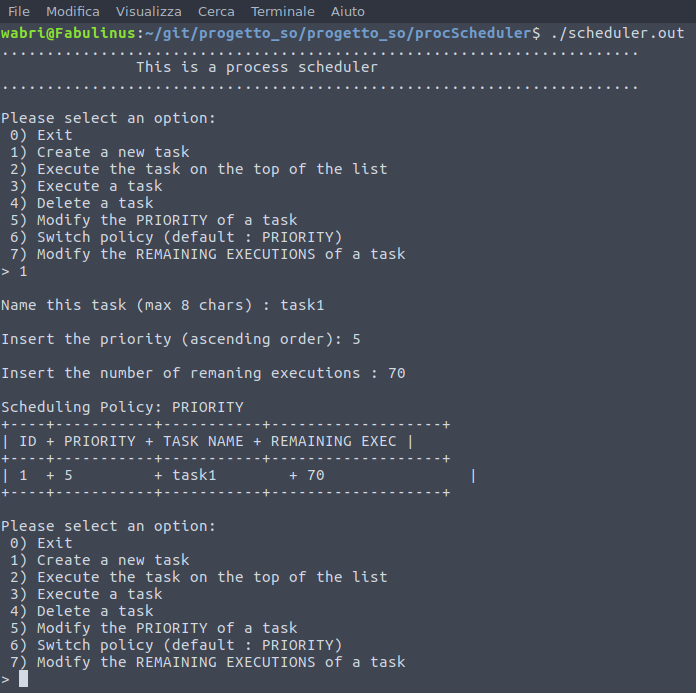
\includegraphics[width=\textwidth]{progetto_so/procScheduler/screenshot/1_new_task_without_error}
\caption{inserimento}
\end{subfigure}
\begin{subfigure}[b]{0.4\textwidth}
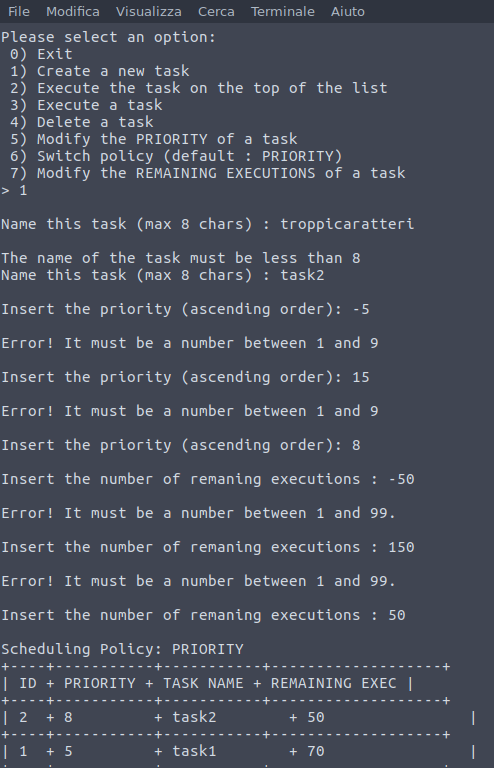
\includegraphics[width=\textwidth]{progetto_so/procScheduler/screenshot/2_new_task_with_error}
\caption{inseriemento con errore}
\end{subfigure}
\begin{subfigure}[b]{0.4\textwidth}
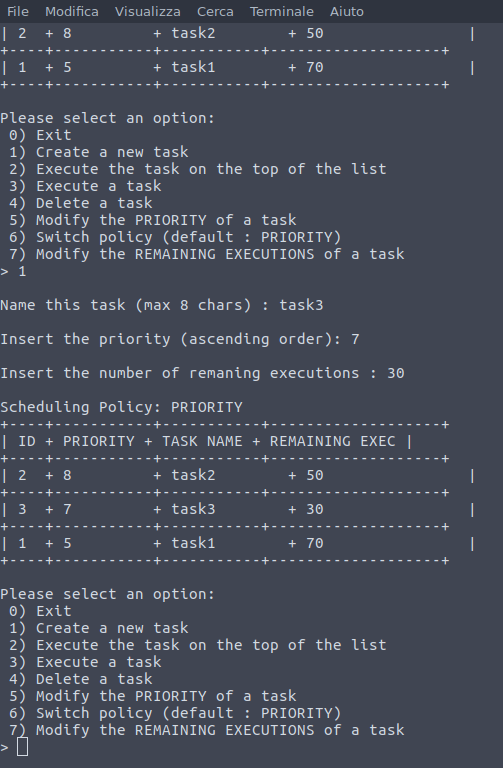
\includegraphics[width=\textwidth]{progetto_so/procScheduler/screenshot/3_new_task_sorting_policy_work}
\caption{inserimento e ordinamento}
\end{subfigure}
\caption{Creazione di un nuovo task}
\end{figure}

\begin{figure}
\centering
\begin{subfigure}[b]{0.4\textwidth}
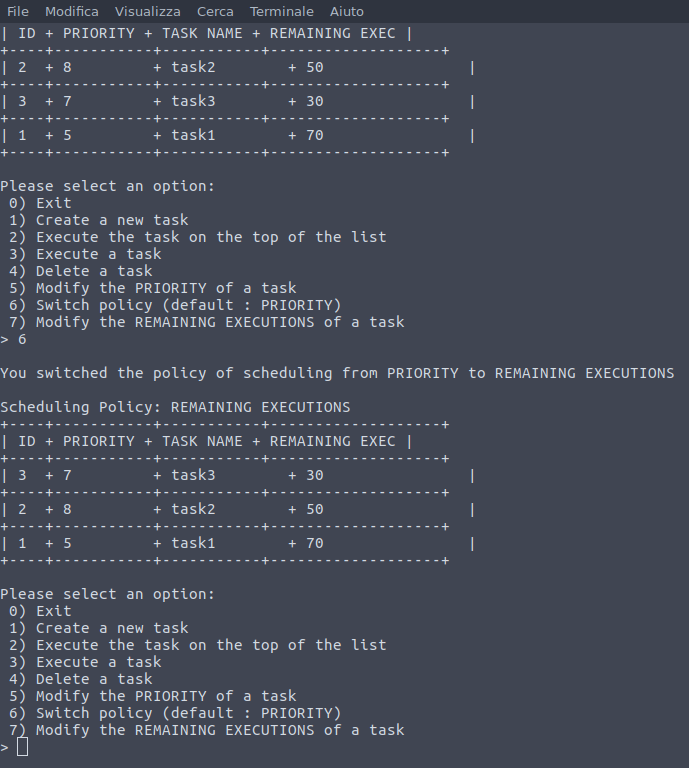
\includegraphics[width=\textwidth]{progetto_so/procScheduler/screenshot/4_change_policy_of_scheduler}
\caption{switch della politica di scheduling}
\end{subfigure}
\begin{subfigure}[b]{0.4\textwidth}
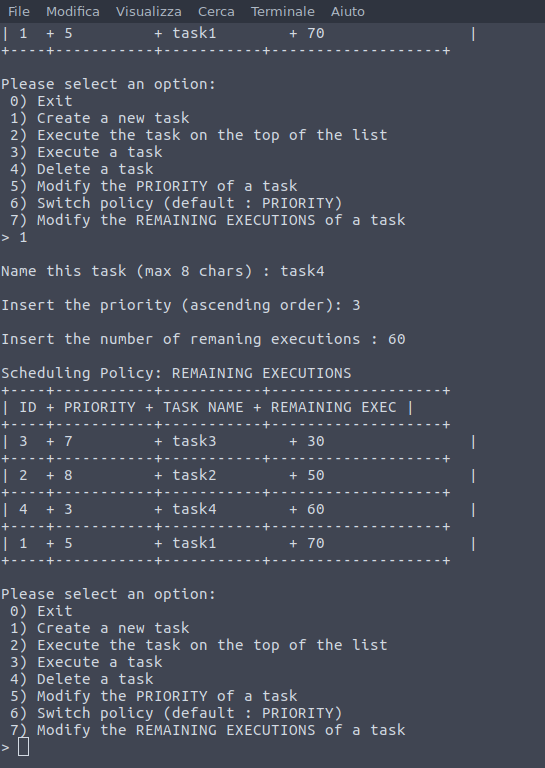
\includegraphics[width=\textwidth]{progetto_so/procScheduler/screenshot/5_new_task_added_to_test_policy_work}
\caption{inserimento e ordinamento}
\end{subfigure}
\begin{subfigure}[b]{0.4\textwidth}
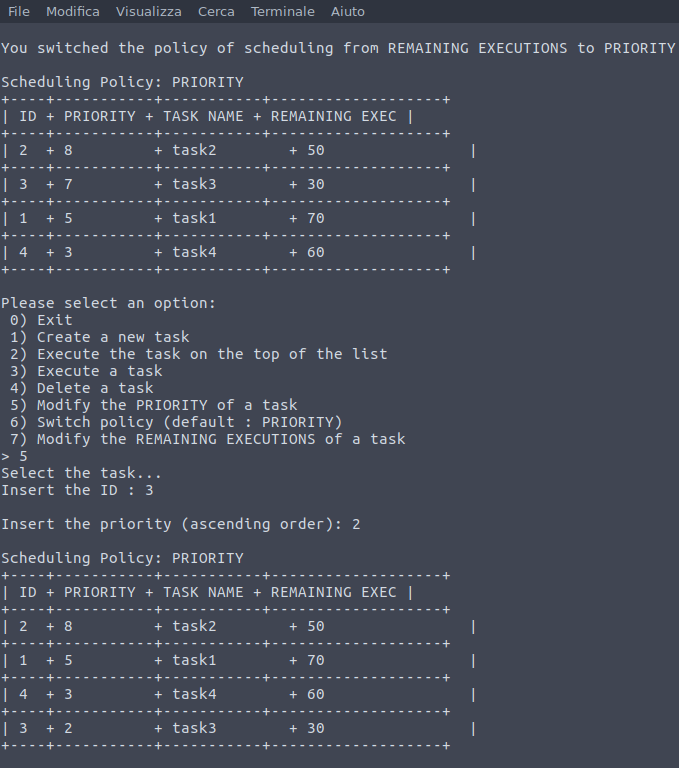
\includegraphics[width=\textwidth]{progetto_so/procScheduler/screenshot/6_switch_policy_and_modify_priority_of_a_task}
\caption{switch della policy e modifica della priori\'a}
\end{subfigure}
\caption{Mantenimento dell'ordinamento della lista dei task e modifica ai parametri}
\end{figure}

\begin{figure}
\centering
\begin{subfigure}[b]{0.4\textwidth}
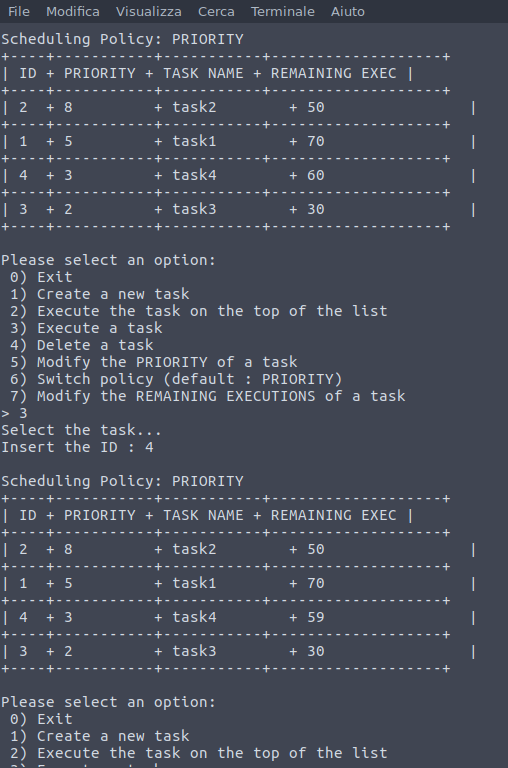
\includegraphics[width=\textwidth]{progetto_so/procScheduler/screenshot/7_single_execution_of_a_task}
\caption{singola esecuzione di un task}
\end{subfigure}
\begin{subfigure}[b]{0.4\textwidth}
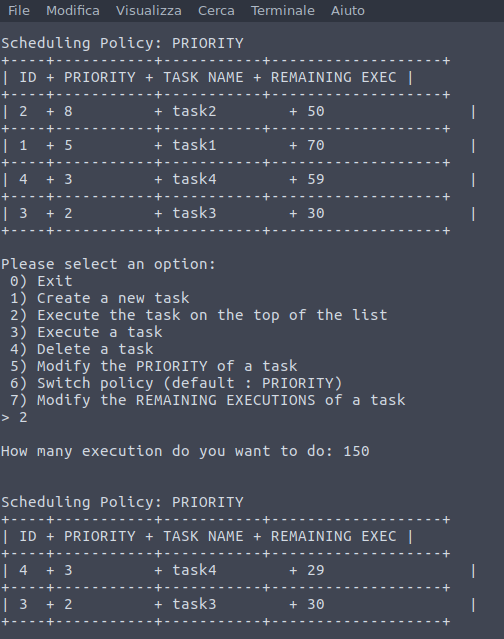
\includegraphics[width=\textwidth]{progetto_so/procScheduler/screenshot/8_150_executions_of_head_tasks}
\caption{150 esecuzioni dei task in testa}
\end{subfigure}
\begin{subfigure}[b]{0.4\textwidth}
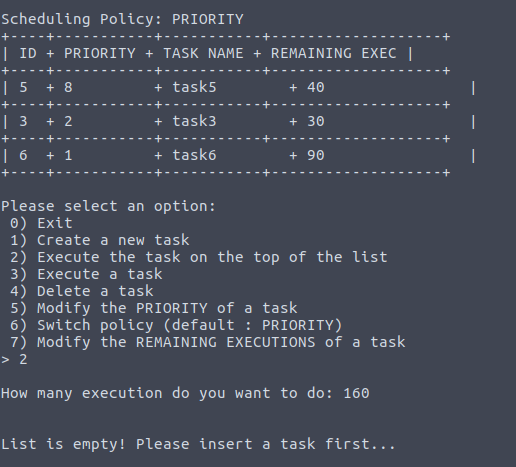
\includegraphics[width=\textwidth]{progetto_so/procScheduler/screenshot/10_execution_of_all_tasks}
\caption{esecuzione di tutti i task}
\end{subfigure}
\caption{Esecuzioni varie dei task}
\end{figure}

\begin{figure}
\centering
\begin{subfigure}[b]{0.4\textwidth}
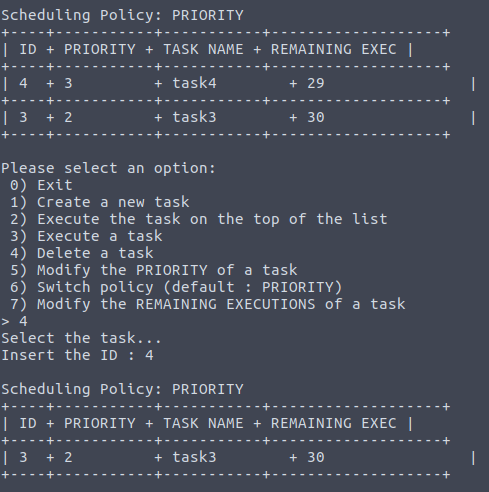
\includegraphics[width=\textwidth]{progetto_so/procScheduler/screenshot/9_deletion_of_a_task}
\caption{eliminazione di tutti i task}
\end{subfigure}
\begin{subfigure}[b]{0.4\textwidth}
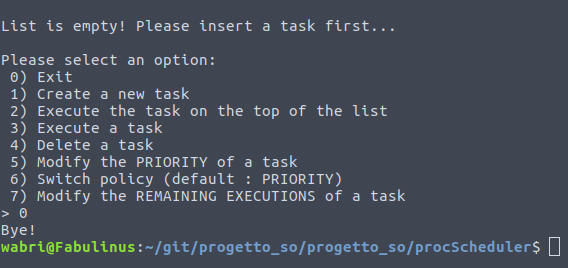
\includegraphics[width=\textwidth]{progetto_so/procScheduler/screenshot/11_exit}
\caption{uscita dal programma}
\end{subfigure}
\caption{Eliminazione dei task ed uscita dal programma}
\end{figure}

\subsubsection{Stress Test}

\begin{figure}[H]
\centering
\begin{subfigure}[b]{0.4\textwidth}
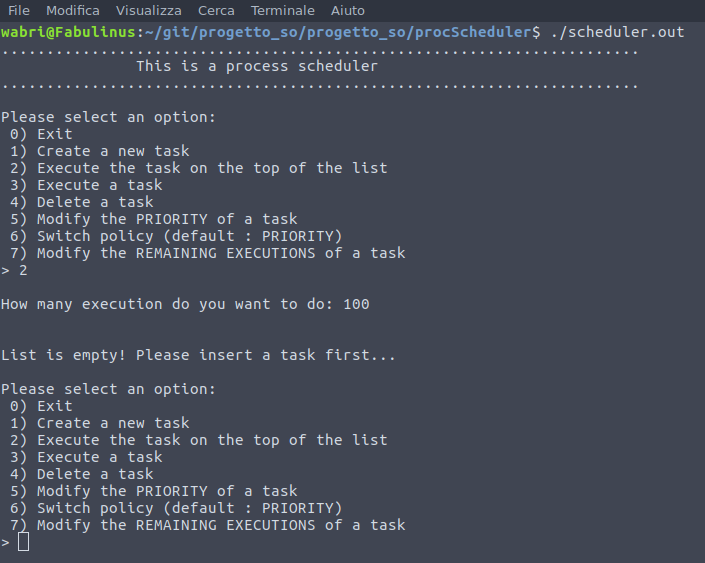
\includegraphics[width=\textwidth]{progetto_so/procScheduler/screenshot/12_stress_test_execute_when_no_tasks_are_in_the_task_list}
\caption{esecuzione a lista vuota}
\end{subfigure}
\begin{subfigure}[b]{0.4\textwidth}
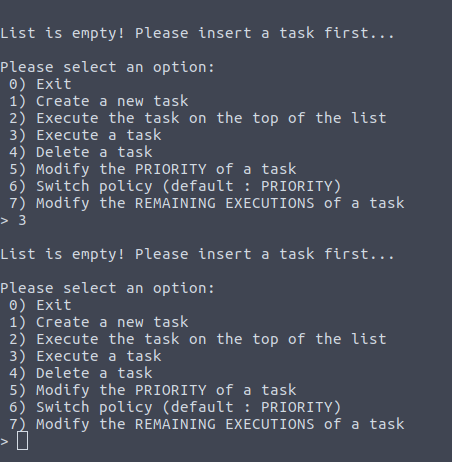
\includegraphics[width=\textwidth]{progetto_so/procScheduler/screenshot/13_stress_test_execute_with_id_when_no_tasks_are_in_the_task_list}
\caption{esecuzione per ID a lista vuota}
\end{subfigure}
\begin{subfigure}[b]{0.4\textwidth}
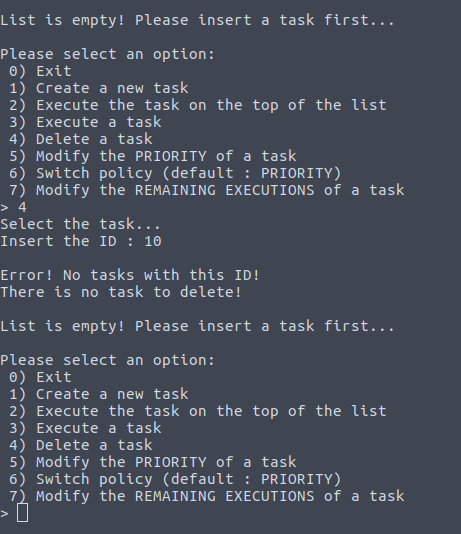
\includegraphics[width=\textwidth]{progetto_so/procScheduler/screenshot/14_stress_test_delete_with_id_when_no_tasks_are_in_the_task_list}
\caption{eliminazione per ID a lista vuota}
\end{subfigure}
\caption{Esecuzioni a lista vuota}
\end{figure}

\begin{figure}
\centering
\begin{subfigure}[b]{0.6\textwidth}
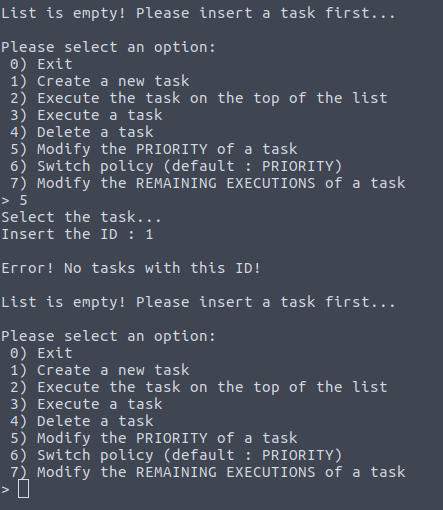
\includegraphics[width=\textwidth]{progetto_so/procScheduler/screenshot/15_stress_test_request_priority_edit_when_no_tasks_are_in_the_list}
\caption{modifica della priorit\'a a lista vuota}
\end{subfigure}
\begin{subfigure}[b]{0.6\textwidth}
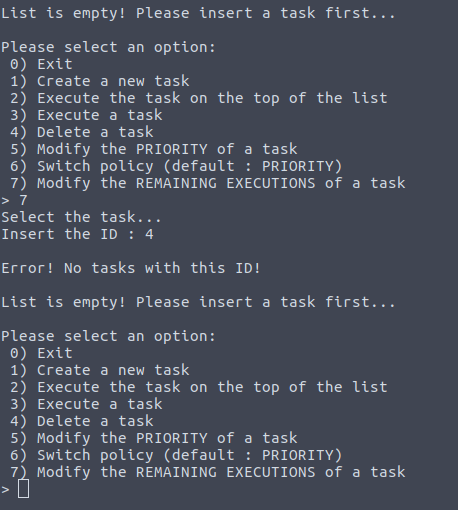
\includegraphics[width=\textwidth]{progetto_so/procScheduler/screenshot/16_stress_test_request_remaining_execution_edit_when_no_tasks_are_in_the_list}
\caption{modifica del n.esec. a lista vuota}
\end{subfigure}
\caption{Modifiche a lista vuota}
\end{figure}

\subsection{Esercizio 2}
\begin{figure}[H]
\centering
\begin{subfigure}[b]{0.8\textwidth}
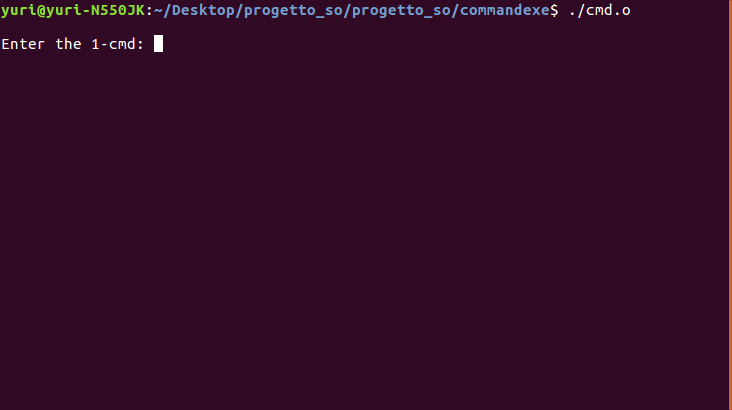
\includegraphics[width=\textwidth]{screencommand/1}
\caption{esecuzioni di \texttt{ls}}
\end{subfigure}
\begin{subfigure}[b]{0.8\textwidth}
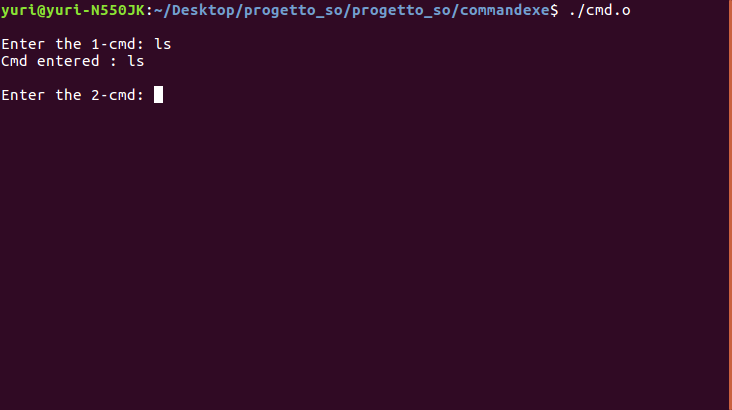
\includegraphics[width=\textwidth]{screencommand/2}
\caption{esecuzioni di \texttt{df -h}}
\end{subfigure}
\end{figure}
\begin{figure}[H]
\centering
\begin{subfigure}[b]{0.8\textwidth}
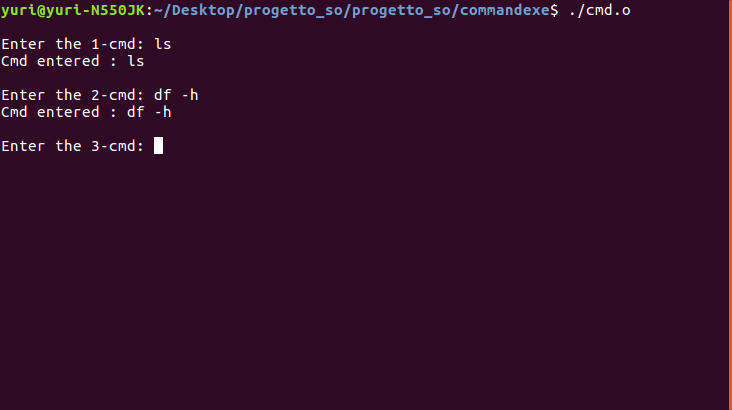
\includegraphics[width=\textwidth]{screencommand/3}
\caption{esecuzioni di \texttt{free}}
\end{subfigure}
\begin{subfigure}[b]{0.8\textwidth}
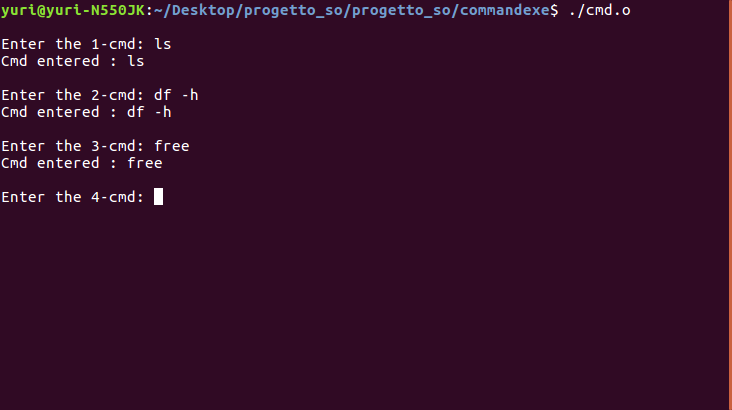
\includegraphics[width=\textwidth]{screencommand/4}
\caption{uscita dal programma}
\end{subfigure}
\end{figure}


\subsection{Esercizio 3}

\begin{itemize}
\item lancio del client con pid 6864 \\
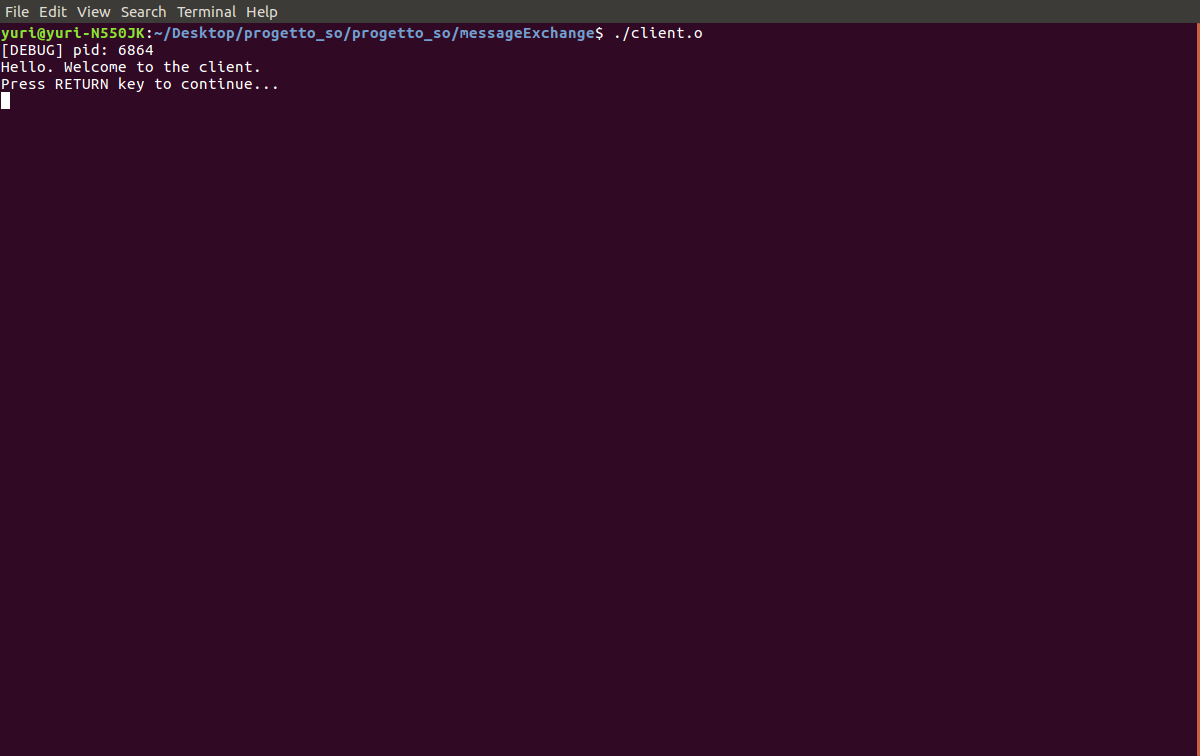
\includegraphics[scale=0.3]{screenmsg/1_client_6864}

\item comparsa del menu \\
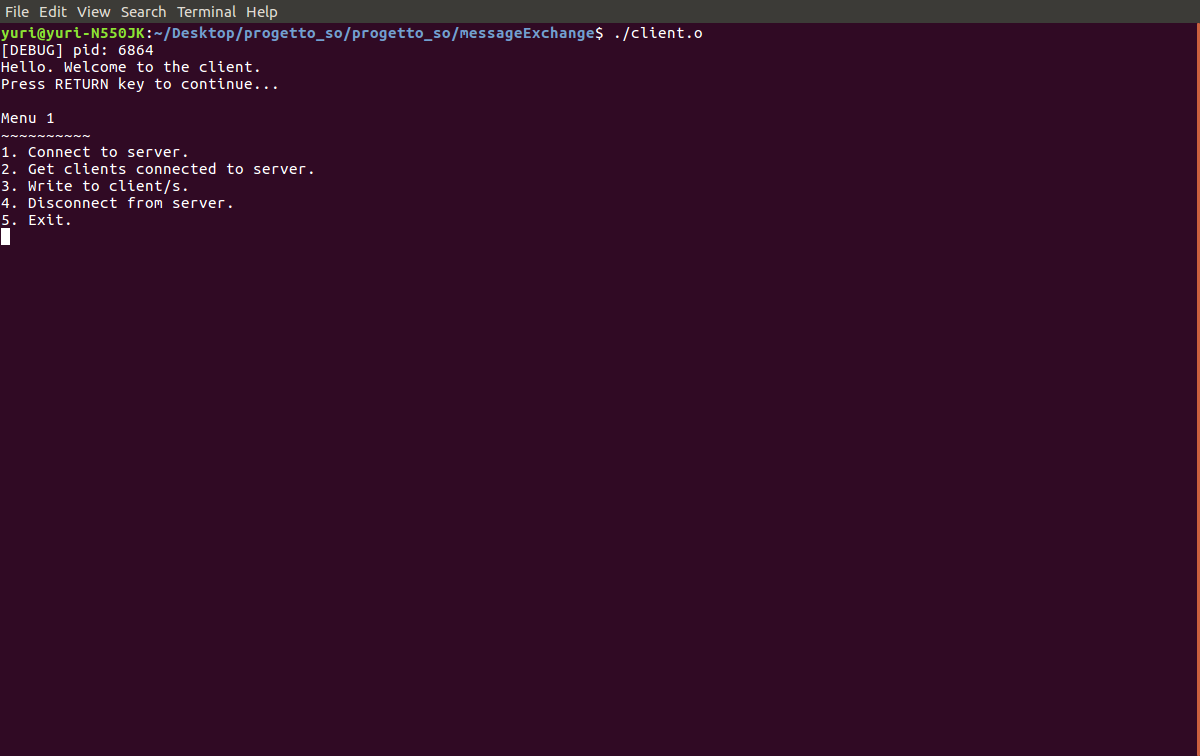
\includegraphics[scale=0.3]{screenmsg/2_client_6864}
\newpage
\item connessione del client 6864 al server \\
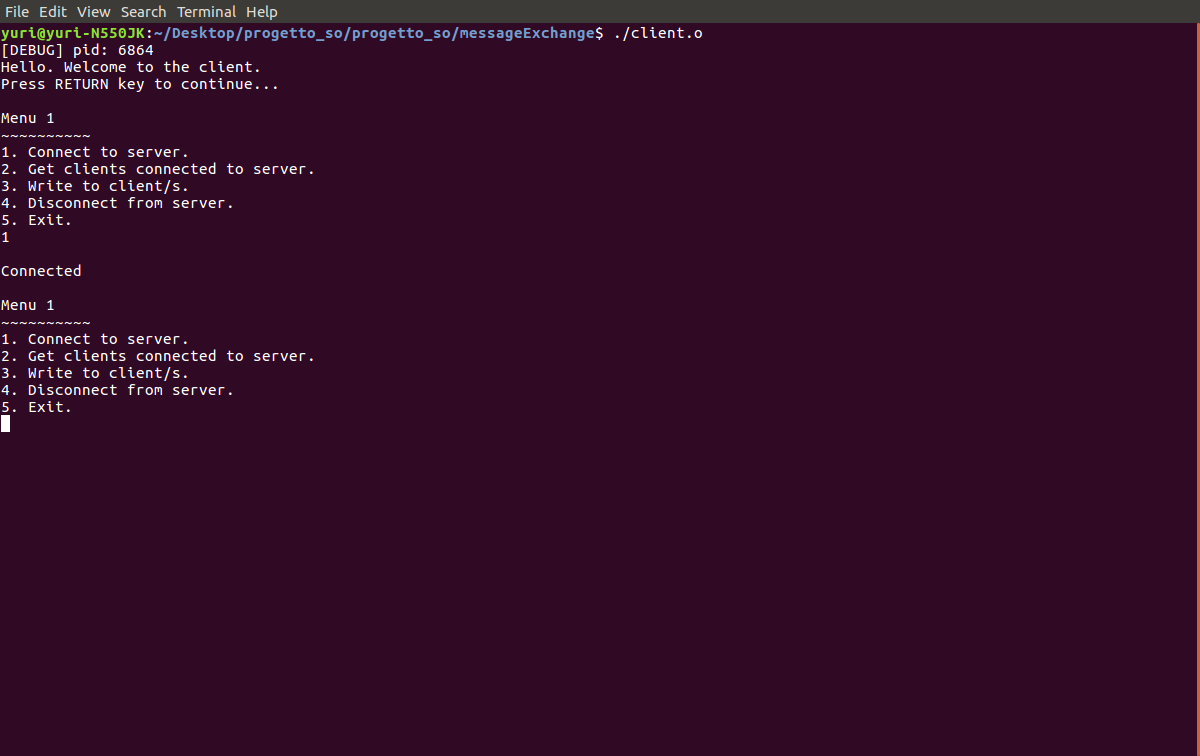
\includegraphics[scale=0.4]{screenmsg/3_client_6864}

\item connessione del client 6932 al server \\
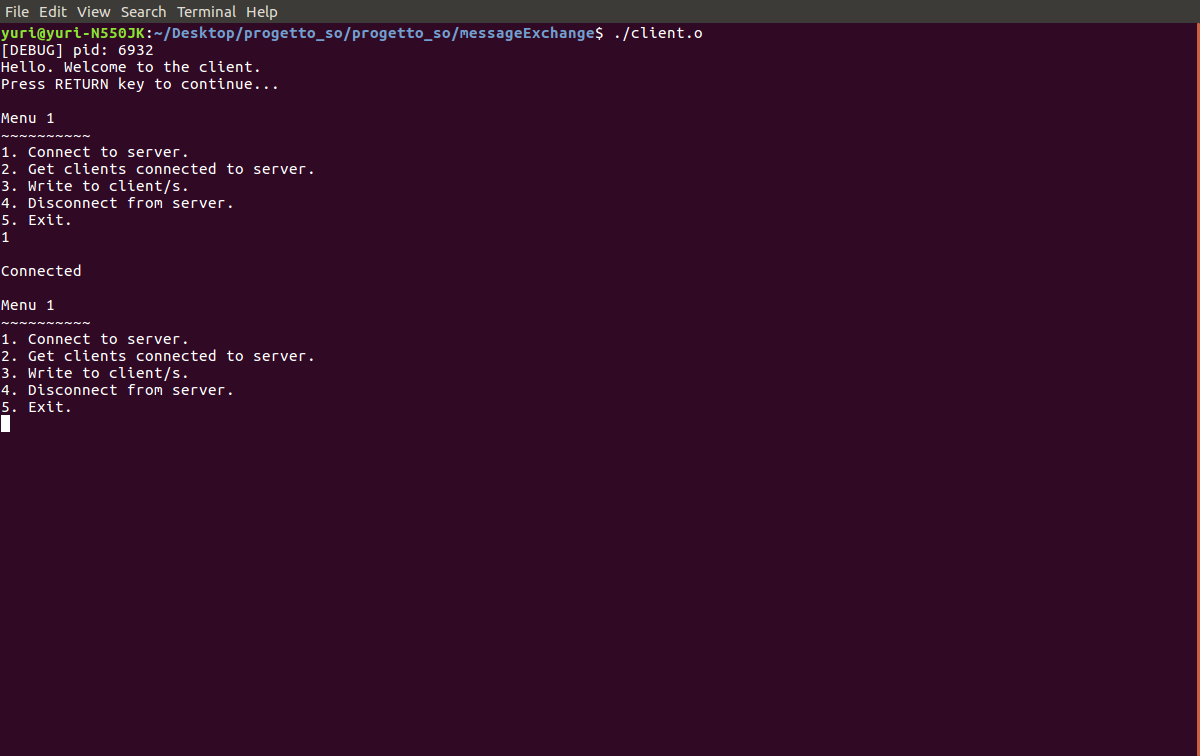
\includegraphics[scale=0.4]{screenmsg/4_client_6932}


\end{itemize}


\begin{figure}[H]
\centering
\begin{subfigure}[b]{0.7\textwidth}
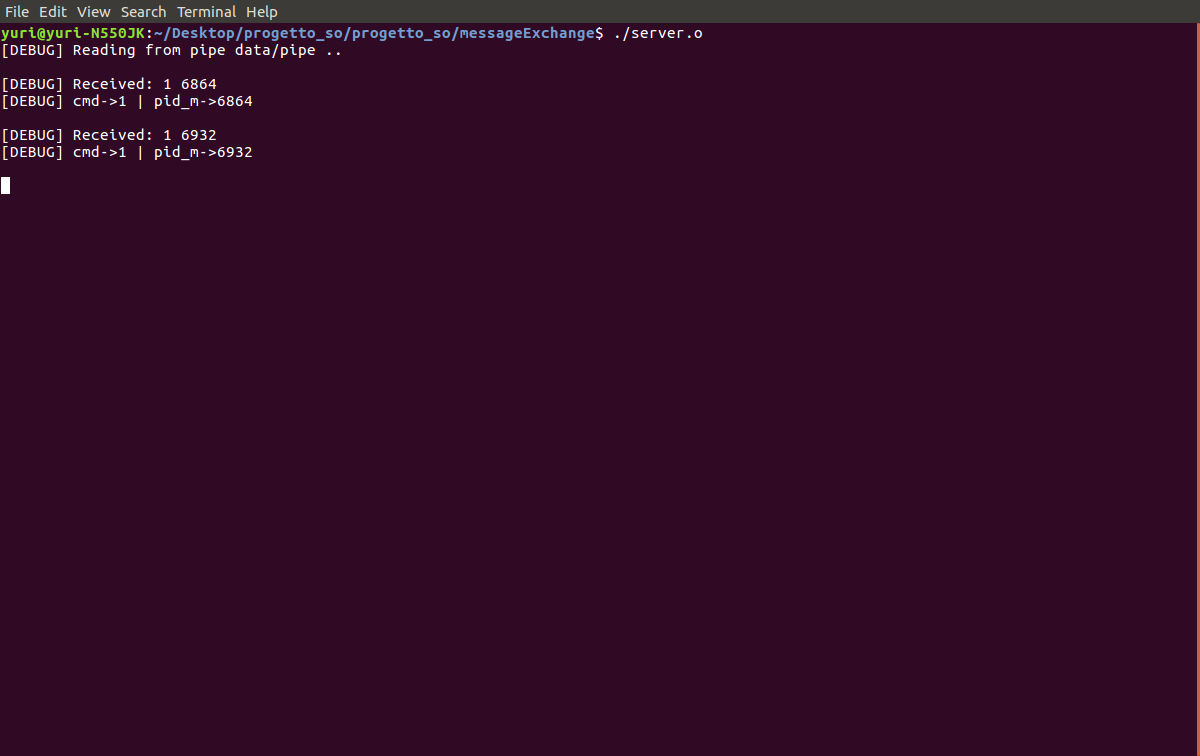
\includegraphics[width=\textwidth]{screenmsg/5_server}
\caption{Connessioni dei client 6864 e 6932 lato server}
\end{subfigure}
\begin{subfigure}[b]{0.7\textwidth}
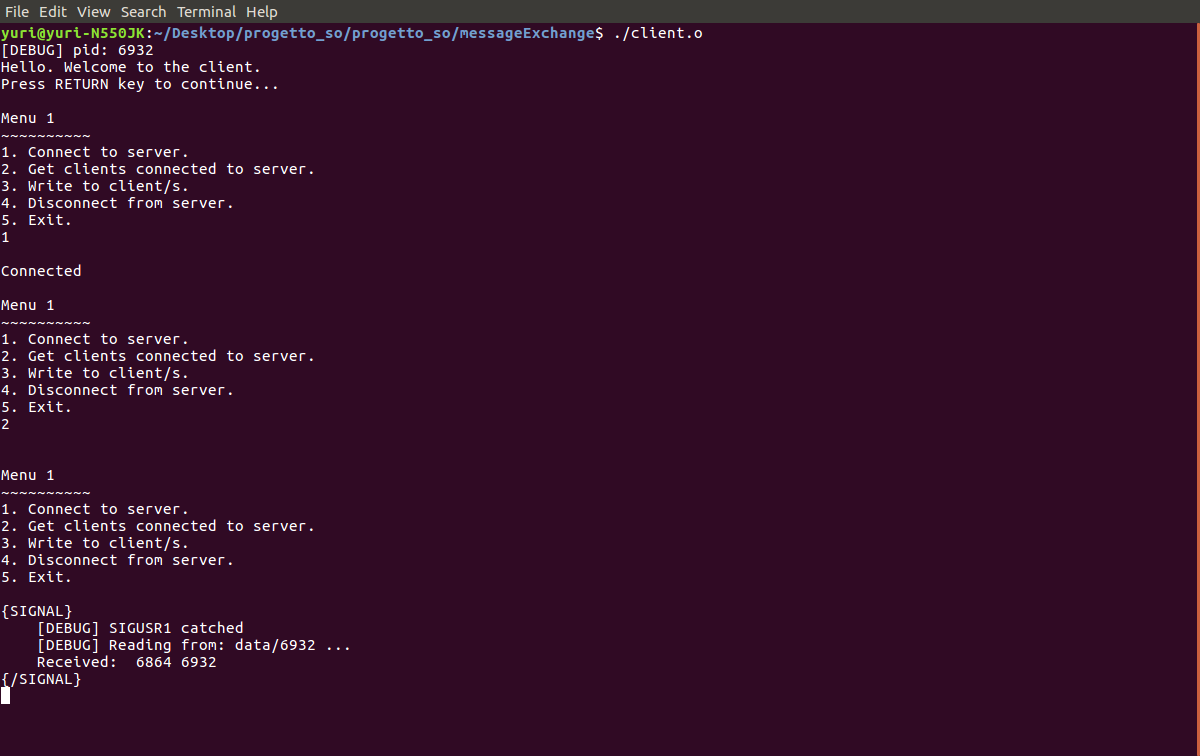
\includegraphics[width=\textwidth]{screenmsg/6_client_6932}
\caption{Richiesta da parte di 6932 dei client connessi}
\end{subfigure}
\begin{subfigure}[b]{0.7\textwidth}
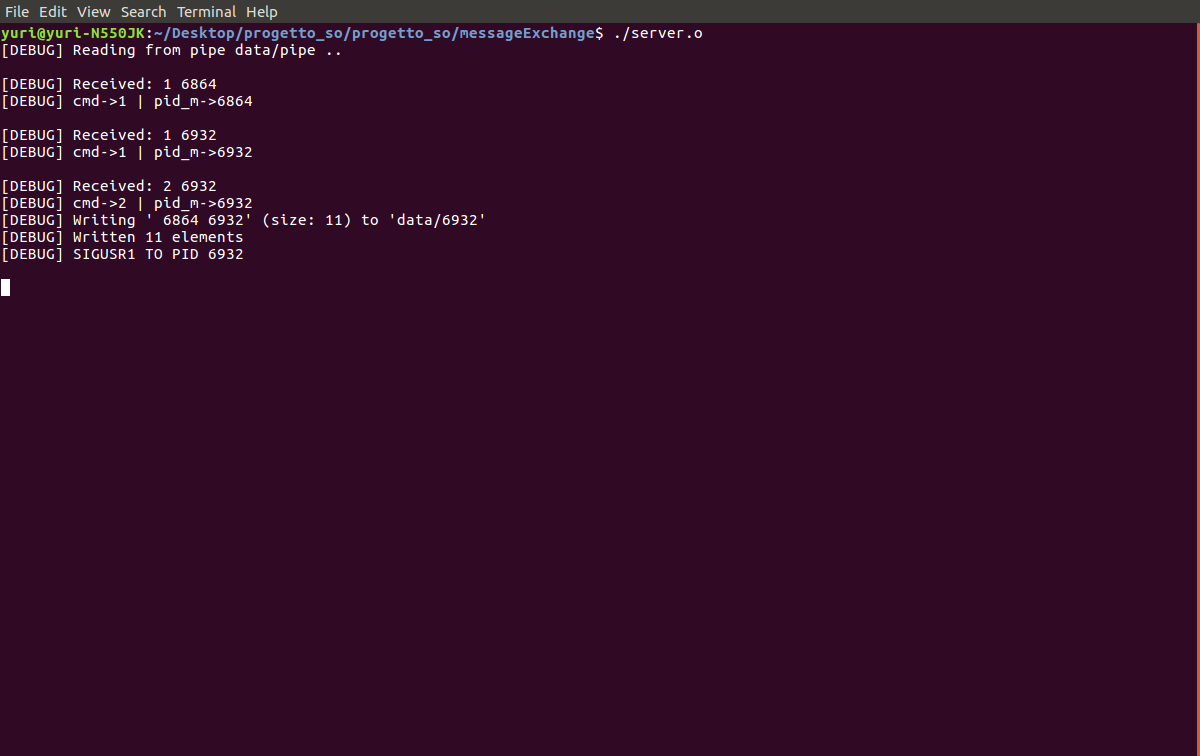
\includegraphics[width=\textwidth]{screenmsg/7_server}
\caption{Risposta del server a 6932}
\end{subfigure}
\caption{Connessioni e richiesta dei client connessi}
\end{figure}

\begin{figure}
\centering
\begin{subfigure}[b]{0.7\textwidth}
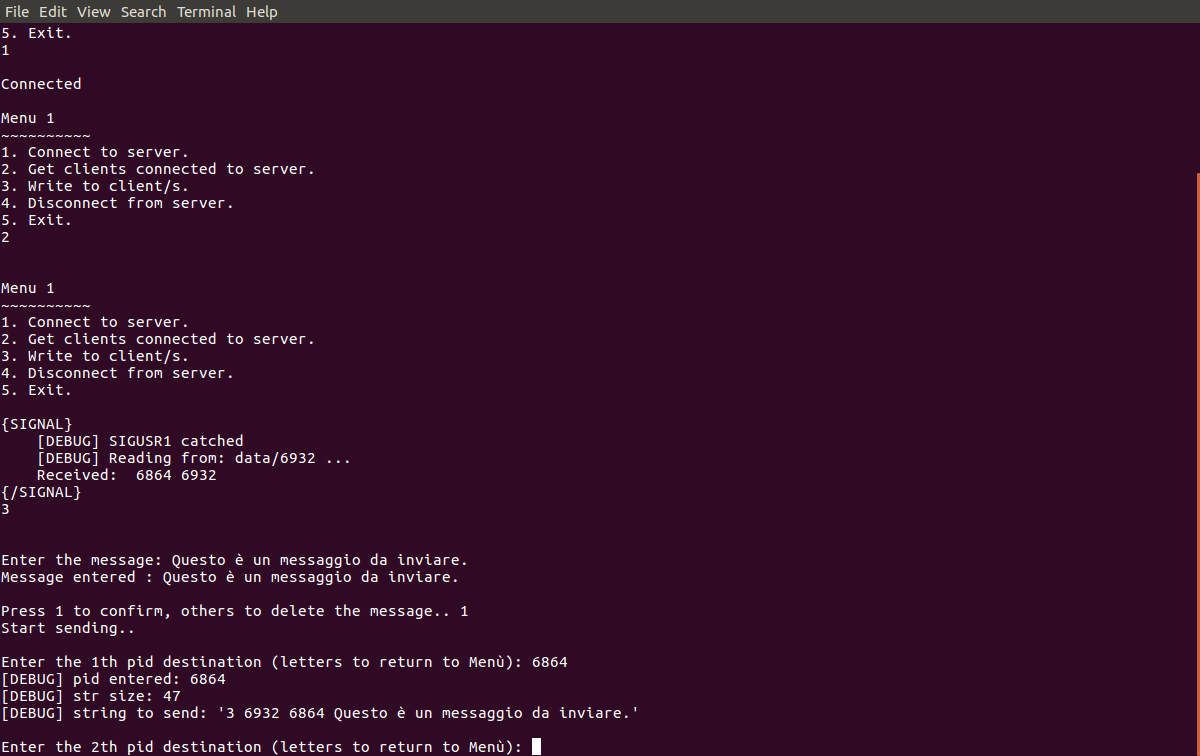
\includegraphics[width=\textwidth]{screenmsg/8_client_6932}
\caption{6932 invia un messaggio a 6864}
\end{subfigure}
\begin{subfigure}[b]{0.7\textwidth}
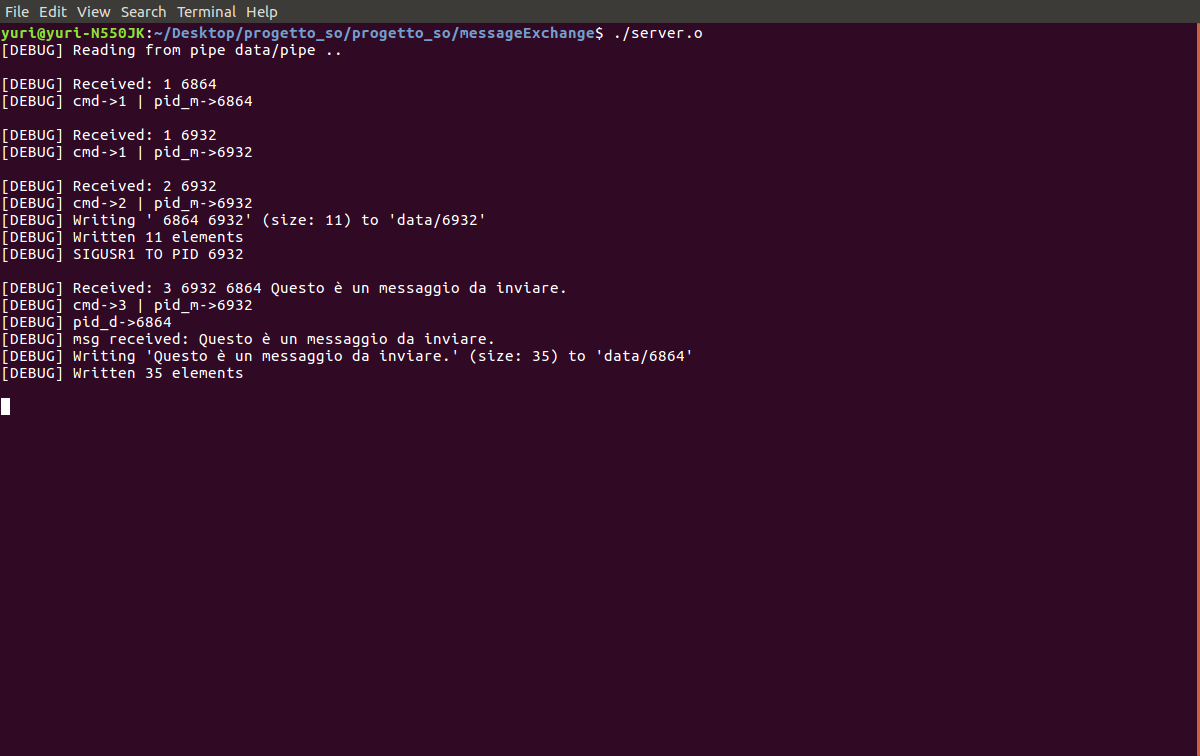
\includegraphics[width=\textwidth]{screenmsg/9_server}
\caption{Risposta del server alla richiesta di 6932}
\end{subfigure}
\begin{subfigure}[b]{0.7\textwidth}
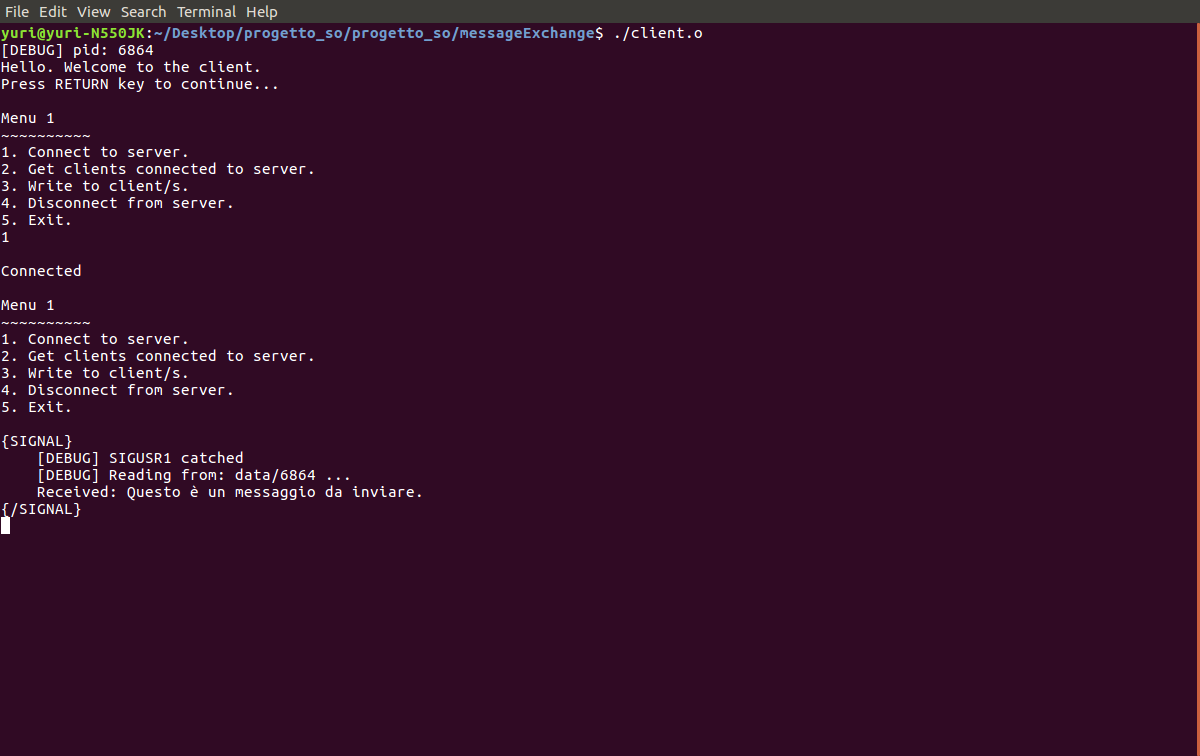
\includegraphics[width=\textwidth]{screenmsg/10_client_6864}
\caption{Ricezione del messaggio da parte di 6864}
\end{subfigure}
\caption{Message passing}
\end{figure}

\begin{figure}
\centering
\begin{subfigure}[b]{0.8\textwidth}
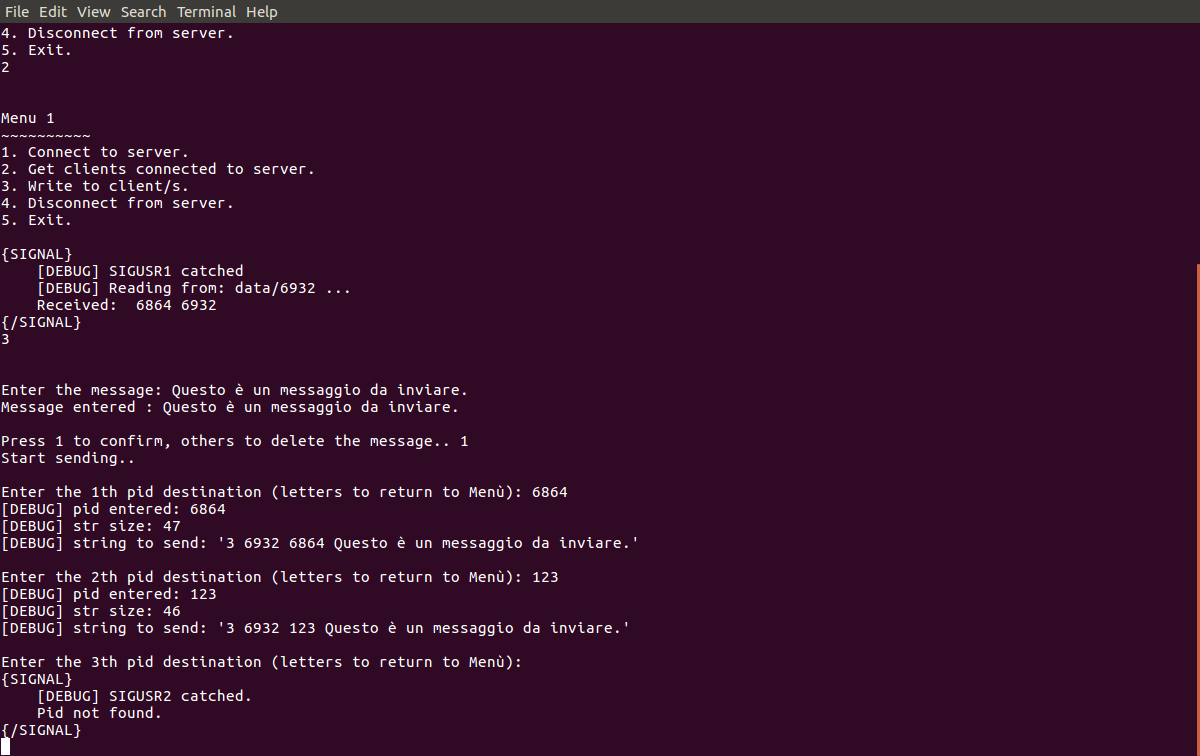
\includegraphics[width=\textwidth]{screenmsg/11_client_6932}
\caption{Gestione dell'errore nell'invio di un messaggio ad un client inesistente}
\end{subfigure}
\begin{subfigure}[b]{0.8\textwidth}
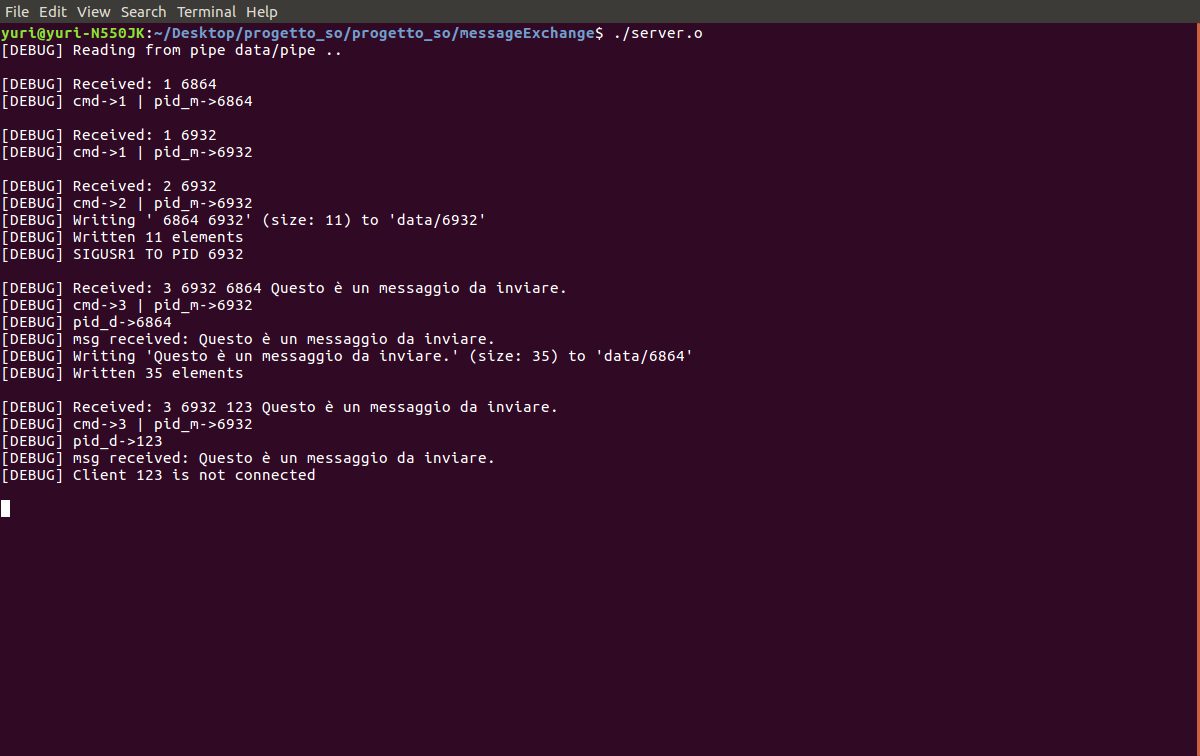
\includegraphics[width=\textwidth]{screenmsg/12_server}
\caption{Gestione dell'errore nell'invio di un messaggio ad un client inesistente lato server}
\end{subfigure}
\caption{Errori}
\end{figure}

\begin{figure}
\centering
\begin{subfigure}[b]{0.7\textwidth}
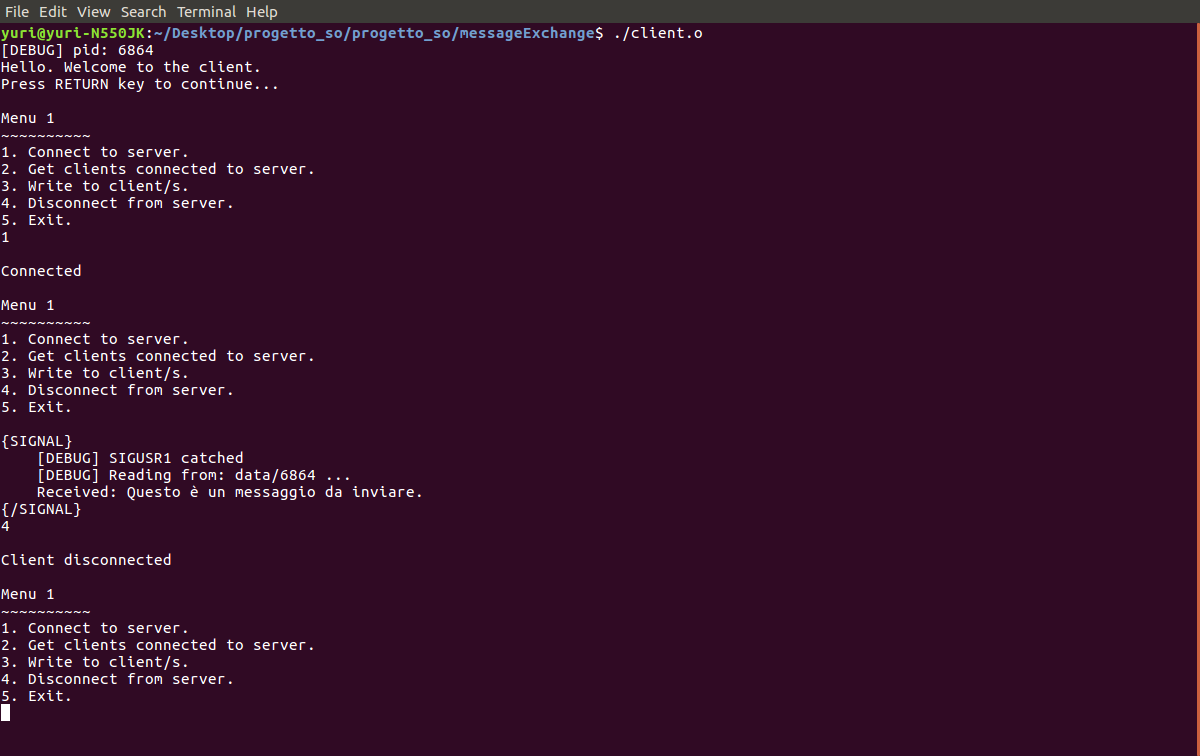
\includegraphics[width=\textwidth]{screenmsg/13_client_6864}
\caption{Disconnessione di 6864 dal server}
\end{subfigure}
\begin{subfigure}[b]{0.7\textwidth}
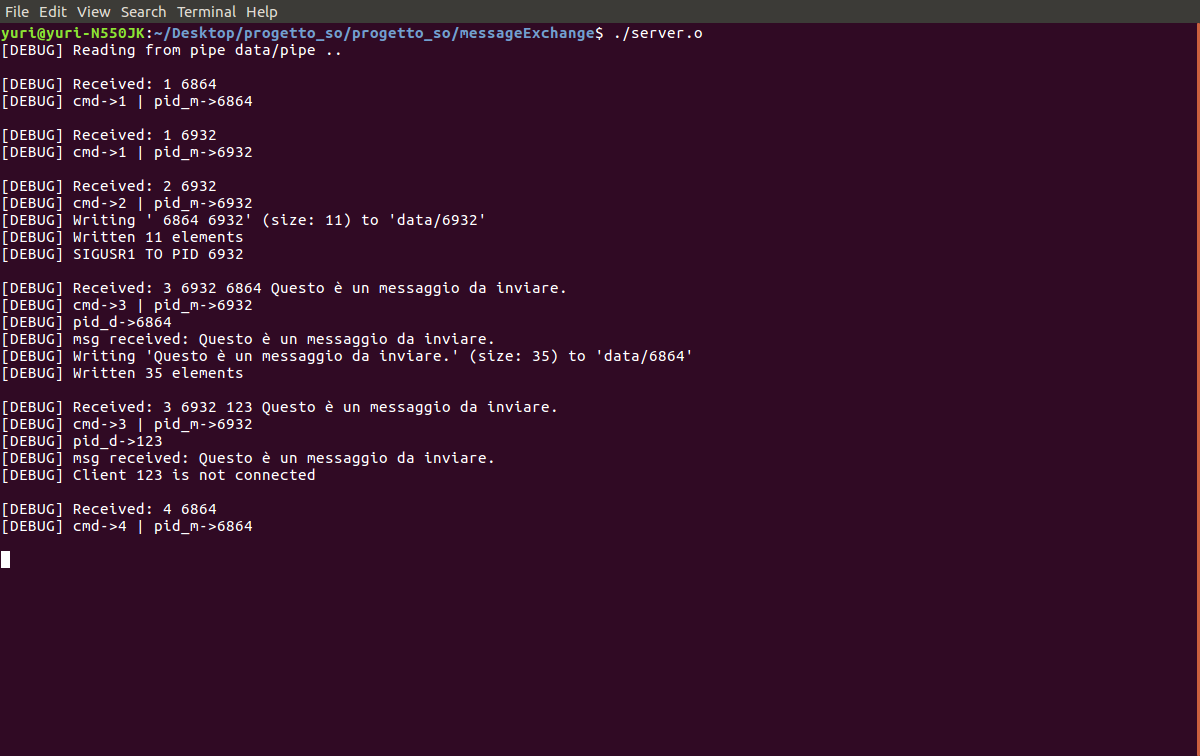
\includegraphics[width=\textwidth]{screenmsg/14_server}
\caption{Risposta del server}
\end{subfigure}
\begin{subfigure}[b]{0.7\textwidth}
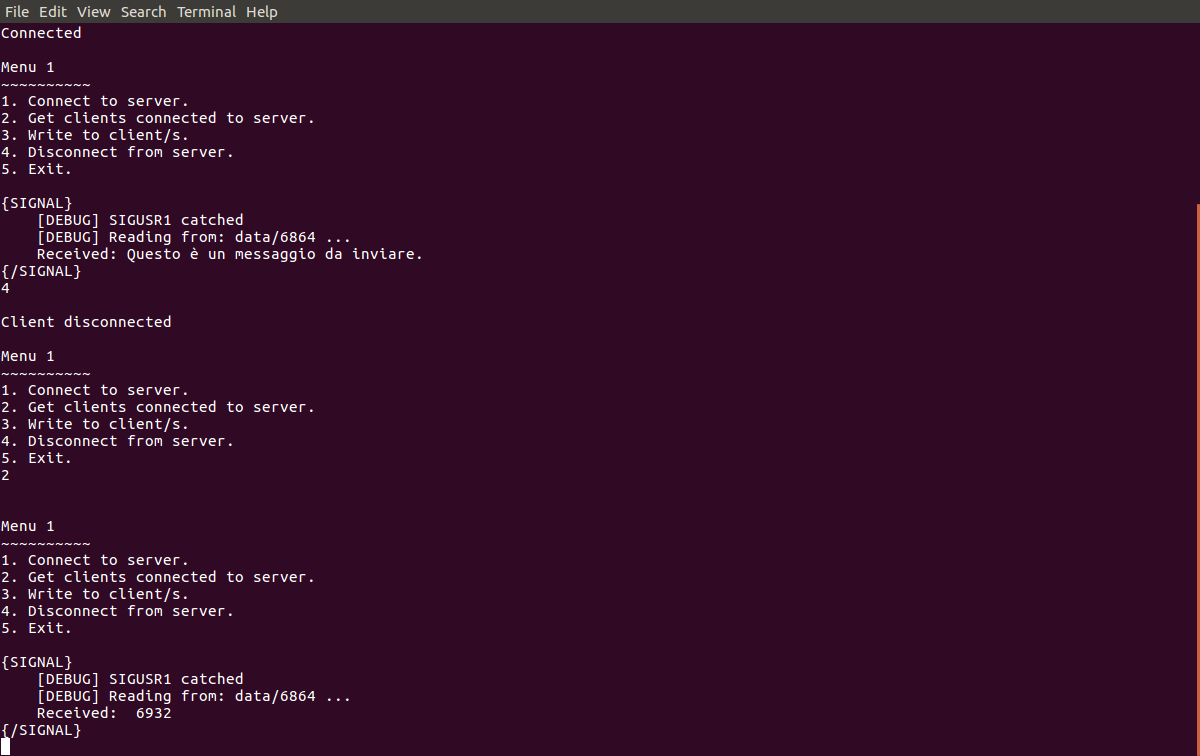
\includegraphics[width=\textwidth]{screenmsg/15_client_6864}
\caption{Richiesta dei client connessi al server}
\end{subfigure}
\caption{Disconnessione}
\end{figure}

\begin{figure}
\centering
\begin{subfigure}[b]{0.8\textwidth}
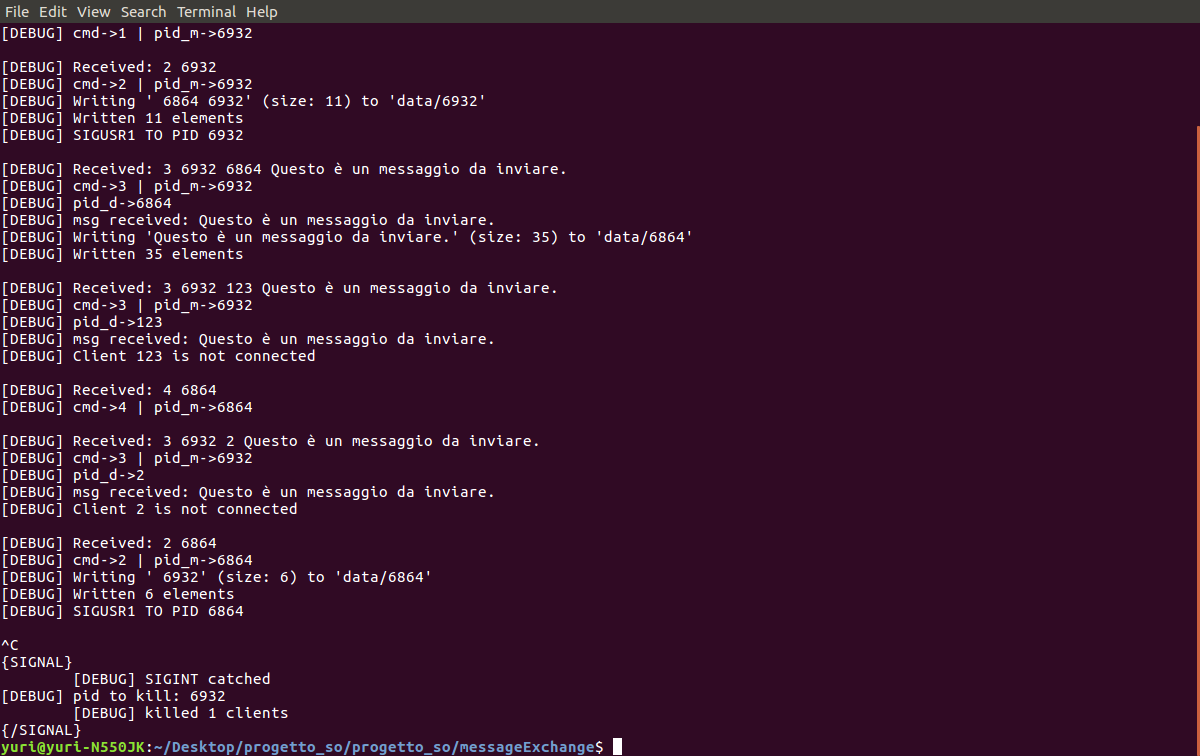
\includegraphics[width=\textwidth]{screenmsg/16_server}
\caption{}
\end{subfigure}
\begin{subfigure}[b]{0.8\textwidth}
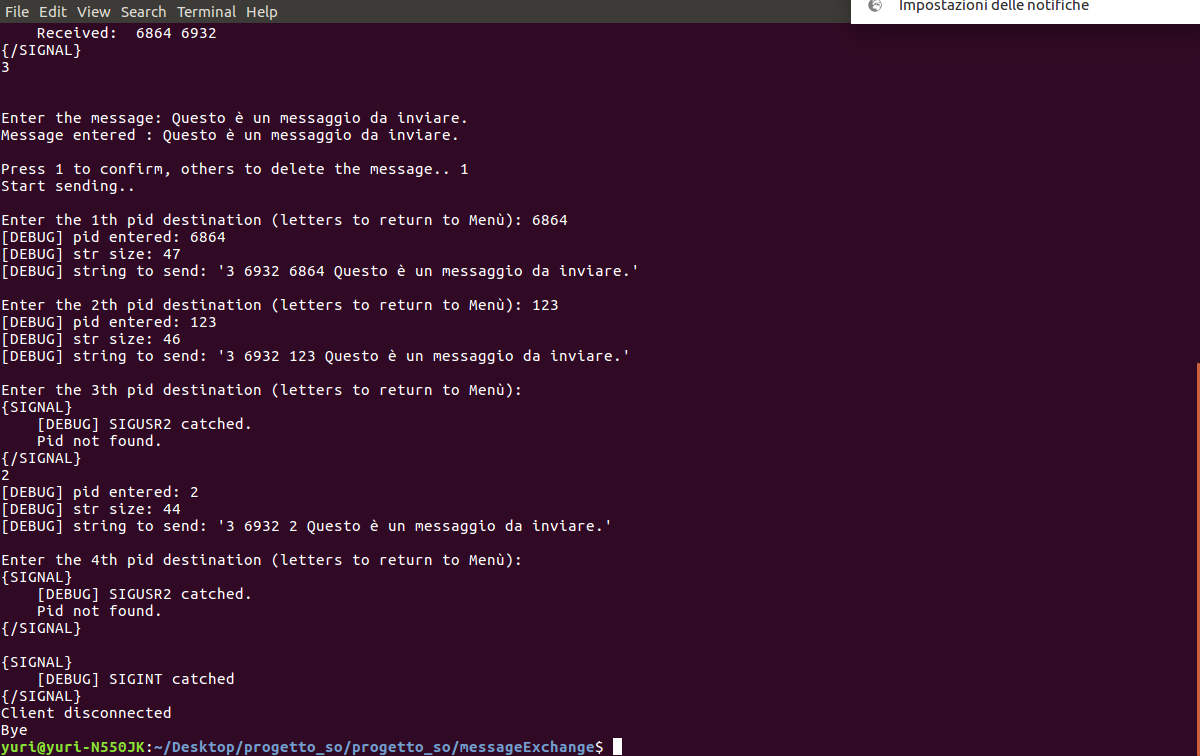
\includegraphics[width=\textwidth]{screenmsg/17_client_6932}
\caption{}
\end{subfigure}
\caption{Errori}
\end{figure}

\end{document}